\documentclass[11pt,a4paper]{article}
\usepackage[a4paper,margin=2.3cm]{geometry}
\usepackage{fontspec}
\setmainfont{Liberation Serif}
\setsansfont{Liberation Sans}
\usepackage{polyglossia}
\setdefaultlanguage{vietnamese}
\usepackage{amsmath,amssymb}
\usepackage{booktabs,tabularx,array,longtable}
\usepackage{graphicx}
\graphicspath{{img/}{../06_code/results/data_story/}}
\usepackage{xcolor}
\usepackage{enumitem}
\usepackage[ruled,vlined,linesnumbered]{algorithm2e}
\usepackage{tikz}
\usetikzlibrary{arrows.meta,positioning,fit}
\usepackage{caption}
\usepackage{hyperref}
\definecolor{teal}{HTML}{0F4C4F}
\definecolor{tealmid}{HTML}{2E7D7A}
\definecolor{tealpale}{HTML}{E6F0EF}
\definecolor{amber}{HTML}{E89B2D}
\definecolor{amberpale}{HTML}{FCF1DF}
\definecolor{coral}{HTML}{C8553D}
\hypersetup{colorlinks=true,linkcolor=teal,urlcolor=tealmid,citecolor=tealmid,pdftitle={Đề xuất Giai đoạn 2: GRAPES-GFN-Rec}}
\newcolumntype{Y}{>{\raggedright\arraybackslash}X}
\setlist{itemsep=2pt,topsep=4pt}
\captionsetup{font=small,labelfont=bf}
\SetAlgorithmName{Thuật toán}{thuật toán}{Danh sách thuật toán}

\title{\textbf{Đề xuất Giai đoạn 2}\\[4pt]\Large GRAPES-GFN-Rec: học cách lấy mẫu đồ thị cho hệ gợi ý quy mô lớn dùng GNN}
\author{Ty Van Xuan}
\date{16 tháng 9 năm 2026}

\begin{document}
\maketitle

\begin{abstract}
\noindent Giai đoạn 1 đã tái hiện GRAPES \cite{grapes} — một phương pháp lấy mẫu đồ thị trong đó một GNN phụ \emph{học} chọn node cho từng layer thông qua GFlowNet — trên bài toán phân loại node. Giai đoạn 2 chuyển ý tưởng này sang hệ gợi ý: đề xuất \textbf{GRAPES-GFN-Rec}, trong đó sampler học chọn node ngữ cảnh cho Sampled LightGCN \cite{lightgcn} và được huấn luyện bằng Trajectory Balance \cite{tb} với phần thưởng từ BPR ranking loss \cite{bpr}. Phương pháp được so sánh với lấy mẫu đều, lấy mẫu theo bậc, biến thể REINFORCE, Full LightGCN, MostPop và BPR-MF dưới cùng graph, budget, seed, evaluator và phần cứng. Dữ liệu chính là Amazon Reviews'23 Baby\_Products \cite{amazon23}: graph huấn luyện có 3.868.654 cạnh, 2.318.308 user, 162.125 item, rất thưa và lệch long-tail. Báo cáo trình bày vấn đề, phân tích dữ liệu, thiết kế phương pháp, protocol đánh giá, rủi ro và kế hoạch triển khai theo tám gate. \textbf{Tại thời điểm viết, chưa có kết quả thực nghiệm nào của GRAPES-GFN-Rec}; phần đã hoàn thành là khóa thiết kế, lõi mã nguồn và bộ kiểm thử oracle.
\end{abstract}

\tableofcontents
\newpage

%=====================================================================
\section{Bối cảnh và động lực}

\subsection{GNN cho hệ gợi ý và bài toán bùng nổ lân cận}
Trong collaborative filtering dựa trên đồ thị, user và item là node, mỗi tương tác là một cạnh. LightGCN \cite{lightgcn} học embedding bằng cách lan truyền và lấy trung bình embedding của hàng xóm qua $L$ bước, không có ma trận biến đổi hay hàm phi tuyến. Để tính embedding của một user ở độ sâu $L$, model cần toàn bộ vùng lân cận $L$ bước của user đó.

Kích thước vùng lân cận tăng theo tích các bậc gặp trên đường đi. Trên graph Baby\_Products, một user trung bình có 1,67 item; nhưng khi đi theo một cạnh ngẫu nhiên, item gặp phải có bậc kỳ vọng
\[
  \mathbb{E}_{\text{cạnh}}[\deg(i)] = \frac{\sum_i \deg(i)^2}{\sum_i \deg(i)} \approx 1.009 \text{ user},
\]
lớn hơn rất nhiều so với bậc trung bình 23,9 của item, vì cạnh dồn vào item phổ biến. Item lớn nhất có 21.348 user. Như vậy chỉ sau hai bước, một user có thể kéo theo hàng nghìn user khác; một batch nhiều triplet hợp các vùng này lại. Đây là hiện tượng \emph{bùng nổ lân cận} (neighbourhood explosion) mà các phương pháp lấy mẫu như GraphSAGE \cite{graphsage}, FastGCN \cite{fastgcn}, LADIES \cite{ladies} và PinSage \cite{pinsage} tìm cách kiểm soát. Kích thước thực tế theo batch và budget sẽ được đo ở gate R3.

\subsection{Lấy mẫu thay đổi thứ model học}
Lấy mẫu giới hạn số node mỗi layer bằng một budget $k$. Đổi lại, model chỉ nhìn thấy một phần ngữ cảnh. Vì vậy sampler không chỉ ảnh hưởng thời gian và bộ nhớ: nó quyết định tín hiệu collaborative mà recommender học được. Câu hỏi \emph{chọn node nào} là câu hỏi nghiên cứu, không chỉ là chi tiết kỹ thuật.

\subsection{Giai đoạn 1: GRAPES}
GRAPES \cite{grapes} dùng hai GNN: $\mathrm{GCN}_C$ giải bài toán chính và $\mathrm{GCN}_S$ chấm điểm hàng xóm để chọn đúng $k$ node mỗi layer bằng Gumbel Top-$k$ \cite{gumbeltopk}. $\mathrm{GCN}_S$ được huấn luyện bằng GFlowNet Trajectory Balance hoặc REINFORCE, với chi phí là loss của $\mathrm{GCN}_C$. Bảng~\ref{tab:phase1} là kết quả tái hiện ở giai đoạn 1 trên Tesla T4.

\begin{table}[h]
\centering\small
\caption{Tái hiện GRAPES ở giai đoạn 1 (accuracy, mean trên các run).}\label{tab:phase1}
\begin{tabular}{lcccc}
\toprule
Dataset & GRAPES & Random & Thời gian GRAPES & Thời gian Random \\
\midrule
Cora & 0,8710 & 0,8677 & 56,3 s & 30,5 s \\
Citeseer & 0,7857 & 0,7900 & 94,6 s & 56,0 s \\
ogbn-arxiv & 0,6204 & 0,6128 & 11.114 s & 8.133 s \\
\bottomrule
\end{tabular}
\end{table}

Hai bài học: (i) sampler học được có thể tốt hơn chọn ngẫu nhiên nhưng lợi thế nhỏ và không đều giữa các dataset; (ii) sampler tốn thêm 37--85\% thời gian, nên chi phí sampler phải nằm trong phép so sánh. GRAPES chỉ được đánh giá trên phân loại node; recommendation được nêu như hướng mở rộng nhưng chưa được kiểm chứng.

\subsection{Rà soát hướng đi trước giai đoạn 2}
Trước khi viết đề xuất này, hướng nghiên cứu đã được rà soát lại. Một nhánh pilot trước đó so sánh ba luật chọn node cố định (M0 đều, M1 theo bậc, M2 frontier-normalized). M2 mượn hình thức hành động của GRAPES (Gumbel Top-$k$, $K^l = V^0 \cup V^l$) nhưng thiếu phần cốt lõi: không có policy học được, không có log-likelihood trajectory, không có phần thưởng, không có mục tiêu TB/REINFORCE và không có bước cập nhật sampler. Vì vậy pilot không trả lời được câu hỏi của đề tài. Quyết định được ghi trong decision log (DL-001): giai đoạn 2 hiện thực một biến thể GRAPES học được, pilot chuyển vào phụ lục.

Để tránh lặp lại, một phương pháp chỉ được gọi là \emph{biến thể GRAPES} nếu thỏa cả bảy điều kiện trong Bảng~\ref{tab:g17}.

\begin{table}[h]
\centering\small
\caption{Checklist G1--G7.}\label{tab:g17}
\begin{tabularx}{\linewidth}{lYc}
\toprule
ID & Thành phần bắt buộc & M2 pilot \\
\midrule
G1 & Policy có tham số ($\mathrm{GCN}_S$ và embedding riêng của sampler) & không \\
G2 & Hành động exact-$k$ bằng Gumbel Top-$k$ trên xác suất của policy & có (trên điểm cố định) \\
G3 & Log-likelihood trajectory $\log q$ & không \\
G4 & Tín hiệu từ loss gợi ý, đã detach & không \\
G5 & Normalizer $\log Z(V^0)$ học được & không \\
G6 & Mục tiêu Trajectory Balance hoặc REINFORCE & không \\
G7 & Tham số sampler thực sự thay đổi qua huấn luyện & không \\
\bottomrule
\end{tabularx}
\end{table}

%=====================================================================
\section{Câu hỏi nghiên cứu}
\textbf{RQ1 (chính).} Trên graph user--item implicit chia theo thời gian, khi giữ cố định recommender, graph, thứ tự triplet BPR, negative, số bước tối ưu, budget node mỗi layer, seed, evaluator và phần cứng, GRAPES-GFN-Rec có đạt trade-off NDCG@20--chi phí huấn luyện tốt hơn lấy mẫu đều và lấy mẫu theo bậc hay không?

\textbf{RQ2.} Trajectory Balance có ổn định hoặc hiệu quả hơn REINFORCE (GRAPES-RL-Rec) trên tín hiệu BPR không?

\textbf{RQ3.} Sampler học được chọn node nào (bậc, loại user/item, nhóm head/body/tail), và điều đó có khuếch đại popularity bias không?

\textbf{RQ4.} Lợi thế, nếu có, thay đổi thế nào khi budget $k$ chặt hơn?

Kết quả âm là kết quả hợp lệ. Nghiên cứu hoàn thành khi trả lời các câu hỏi với bằng chứng truy vết được, không phụ thuộc vào việc GRAPES-GFN-Rec thắng.

%=====================================================================
\section{Dữ liệu}

\subsection{Chọn dataset}
Amazon Reviews'23 \cite{amazon23} có nhiều danh mục, số giao dịch lớn và metadata sản phẩm có thể nối thêm. Ba danh mục đã được kiểm toán chính xác trên file tải về:

\begin{table}[h]
\centering\small
\caption{Portfolio dữ liệu Amazon đã kiểm toán.}\label{tab:datasets}
\begin{tabularx}{\linewidth}{lrY}
\toprule
Dataset & Dòng raw & Vai trò \\
\midrule
All\_Beauty & 693.929 & Kiểm tra pipeline; quá nhỏ, chỉ 3,98\% target validation còn warm-start. \\
Baby\_Products & 5.953.891 & \textbf{Dữ liệu chính}: 3,39 triệu user, 217.654 item; đủ lớn để thấy chi phí sampling, long-tail rõ, chạy được ma trận thí nghiệm trên Colab T4. \\
Home\_and\_Kitchen & 66.623.880 & Tham chiếu quy mô (11,2 lần Baby); dành cho stress test sau khi có kết quả Baby. \\
\bottomrule
\end{tabularx}
\end{table}

MovieLens 25M, Gowalla, Yelp2018, MIND và KuaiRec đã được cân nhắc. Chúng phù hợp các câu hỏi khác — dữ liệu có nội dung, exposure gần đầy đủ, hoặc split ngẫu nhiên đã xử lý sẵn — nên chỉ dùng làm bối cảnh, chưa chạy thực nghiệm.

\subsection{Chất lượng và nhiễu}
Kiểm toán Baby\_Products cho thấy không có dòng thiếu ID, không có timestamp sai và không có cặp user--item trùng. Chỉ có một dòng rating $0.0$ ngoài miền 1--5; dòng này bị loại. Phân bố rating lệch mạnh về 5 sao (Bảng~\ref{tab:rating}). Quy tắc P4 xem rating 4--5 là tương tác positive, giữ 4.655.843 dòng (78,20\%).

\begin{table}[h]
\centering\small
\caption{Phân bố rating Baby\_Products.}\label{tab:rating}
\begin{tabular}{lrrrrrr}
\toprule
Rating & 0 & 1 & 2 & 3 & 4 & 5 \\
\midrule
Số dòng & 1 & 555.424 & 309.591 & 433.032 & 681.977 & 3.973.866 \\
\bottomrule
\end{tabular}
\end{table}

Không lọc $k$-core: lọc sẽ xóa đúng phần long-tail và user ít tương tác mà bài toán lấy mẫu cần đối mặt.

\subsection{Mất cân bằng và long-tail}
\begin{figure}[h]
\centering
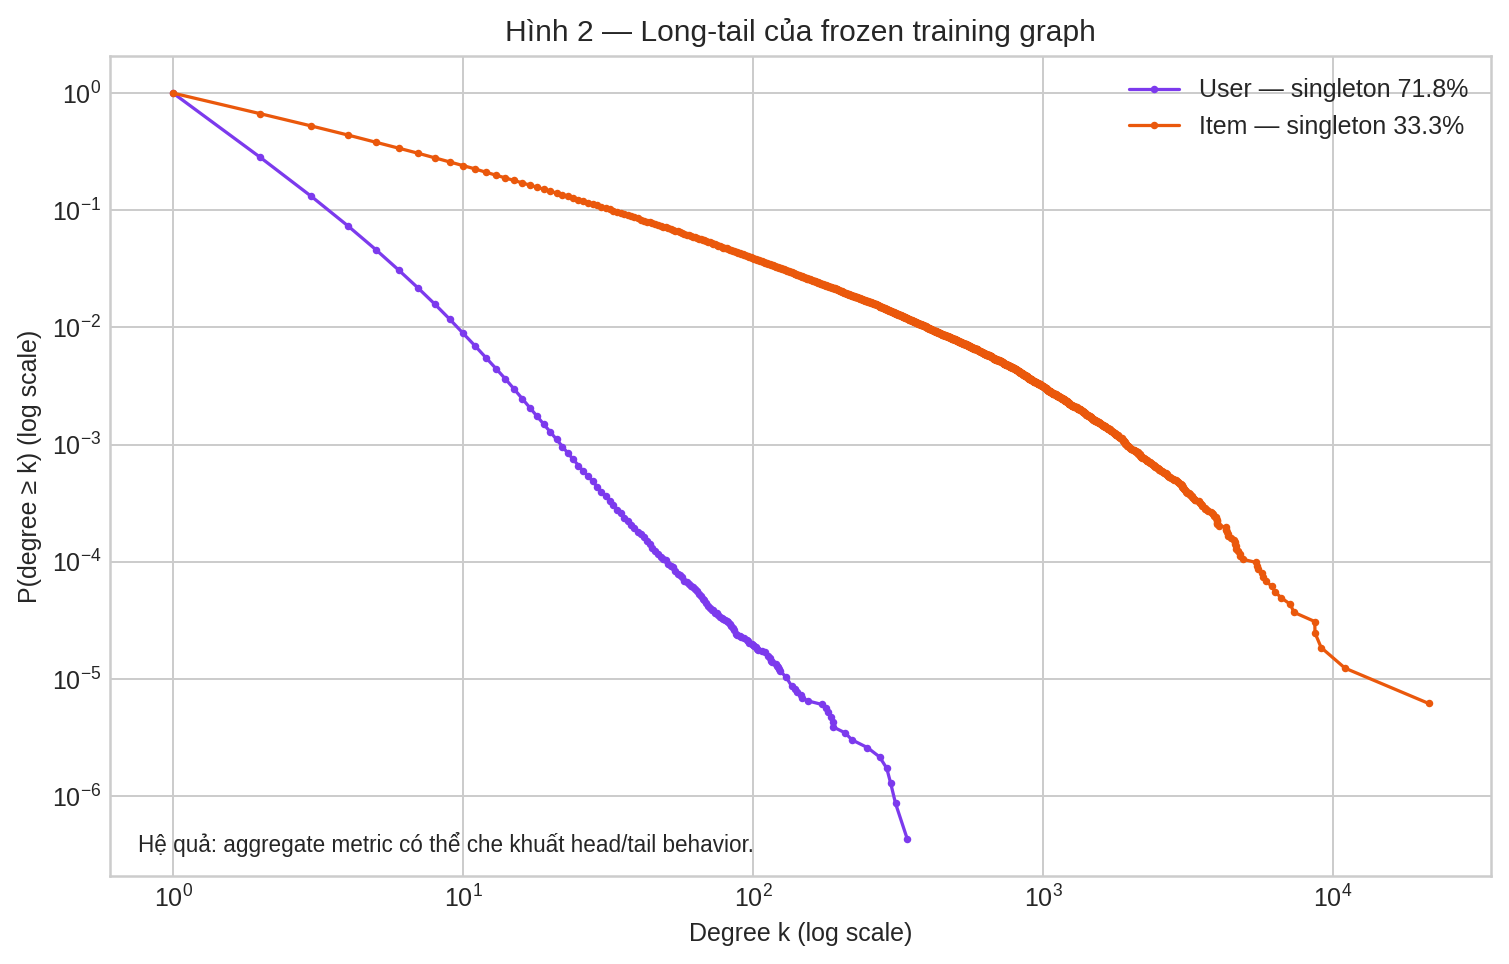
\includegraphics[width=0.49\linewidth]{02_degree_long_tail.png}\hfill
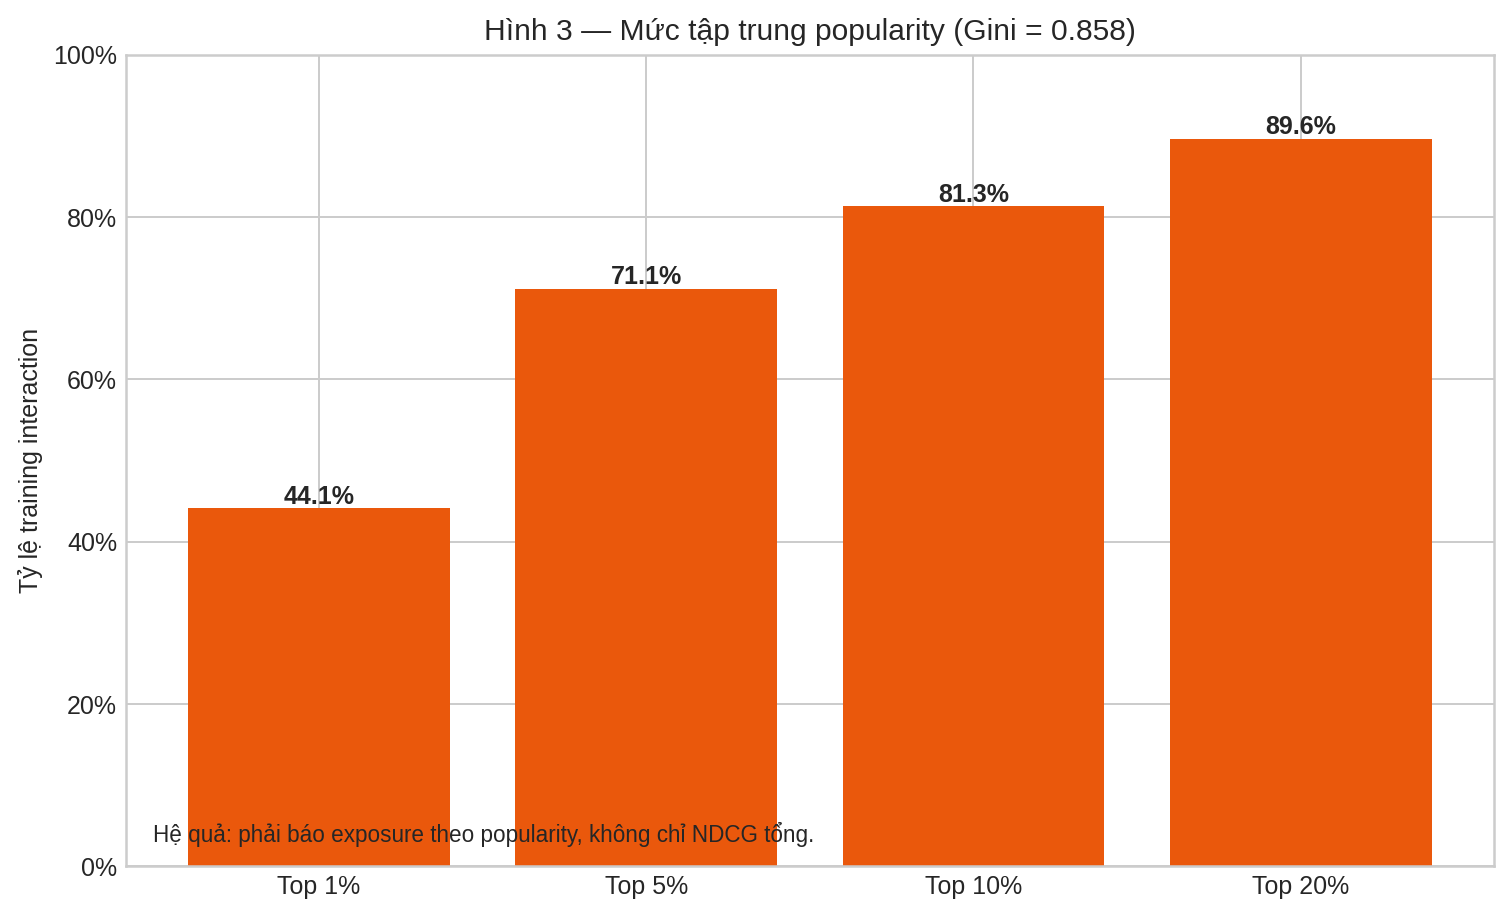
\includegraphics[width=0.49\linewidth]{03_item_concentration.png}
\caption{Trái: phân phối bậc user và item (log--log). Phải: tỷ lệ tương tác do item phổ biến nhất nắm giữ.}\label{fig:longtail}
\end{figure}

Graph huấn luyện rất thưa (mật độ $1{,}03\times10^{-5}$) và lệch (Hình~\ref{fig:longtail}):
\begin{itemize}
\item 71,76\% user chỉ có một tương tác; bậc user p50/p90/p99 = 1/3/9.
\item 33,35\% item chỉ có một tương tác; bậc item p50/p90/p99 = 3/32/397; Gini bậc item 0,8584.
\item Top 1\% item giữ 44,09\% tương tác; top 20\% giữ 89,65\%.
\end{itemize}

Hệ quả cho thiết kế: (i) điểm tổng có thể tăng chỉ nhờ phục vụ tốt item phổ biến, nên phải báo exposure và hit theo head/body/tail; (ii) user gần như không có ngữ cảnh riêng, nên lựa chọn của sampler có ý nghĩa chủ yếu ở layer đi qua item; (iii) sampler học được có thể dồn về hub, nên phải theo dõi bậc và nhóm của node được chọn.

\subsection{Đường đi dữ liệu và chia theo thời gian}
Pipeline: raw CSV (kiểm SHA-256) $\rightarrow$ kiểm toán $\rightarrow$ P4 $\rightarrow$ chia theo thời gian $\rightarrow$ graph train và mapping ID $\rightarrow$ huấn luyện có lấy mẫu $\rightarrow$ đánh giá full-graph, full-catalog.

Hai mốc hiện có là $t_1$ = 11/08/2021 và $t_2$ = 16/07/2022. Graph train chỉ gồm cạnh trước $t_1$. Validation gồm 81.871 target warm-start trong $[t_1, t_2)$; test gồm 40.587 target sau $t_2$ và chưa được đọc. Vì validation đã bị pilot quan sát, giai đoạn 2 tạo một \emph{development split} mới:
\[
t_0 = t_1 - (t_2 - t_1), \qquad G_{\text{dev\_train}} = \{e : ts(e) < t_0\}, \qquad D_{\text{dev}} = \{e : t_0 \le ts(e) < t_1,\ \text{warm-start}\}.
\]
Nếu $D_{\text{dev}}$ có dưới 20.000 target hoặc $G_{\text{dev\_train}}$ mất quá 50\% cạnh, dùng quy tắc dự phòng đã đăng ký: chọn $t_0$ sao cho $G_{\text{dev\_train}}$ giữ 80\% cạnh. Vai trò các split nêu ở Bảng~\ref{tab:splits}.

\begin{table}[h]
\centering\small
\caption{Vai trò các split.}\label{tab:splits}
\begin{tabularx}{\linewidth}{lYY}
\toprule
Split & Dùng cho & Cấm \\
\midrule
$G_{\text{dev\_train}}$ / $D_{\text{dev}}$ & Chọn budget, $\alpha$, learning rate, kiến trúc sampler; kiểm tra backbone & Kết luận cuối \\
Graph train / validation & So sánh ghép cặp sau khi freeze cấu hình & Mọi điều chỉnh \\
Test & Một lần, nếu có protocol final-test riêng & Chọn phương pháp \\
\bottomrule
\end{tabularx}
\end{table}

Cạnh tương lai không được đi vào graph, degree, tập ứng viên, feature của sampler, normalization hay hàm mục tiêu.

%=====================================================================
\section{Phương pháp đề xuất: GRAPES-GFN-Rec}

\subsection{Kiến trúc tổng thể}
\begin{figure}[h]
\centering
\begin{tikzpicture}[
  node distance=0.5cm and 0.35cm,
  b/.style={draw=none,rounded corners=3pt,fill=tealpale,align=center,font=\sffamily\small,minimum height=1.0cm,text width=2.2cm},
  d/.style={b,fill=teal,text=white},
  o/.style={b,fill=amberpale},
  a/.style={b,fill=amber},
  ar/.style={-{Stealth[length=2.5mm]},thick,gray}]
\node[b] (batch) {Batch BPR\\$(u,i^+,i^-)$};
\node[b,right=of batch] (v0) {$V^0$ = tập\\endpoint};
\node[d,right=of v0,text width=3.6cm] (s) {Sampler $\mathrm{GCN}_S$\\\mbox{Gumbel Top-$k$}\\mỗi layer};
\node[d,right=of s,text width=3.3cm] (r) {Sampled LightGCN\\trên $K^1,\dots,K^L$};
\node[o,below=of r,text width=3.3cm] (bpr) {BPR loss\\$\rightarrow$ cập nhật $\Theta_R$};
\node[b,below=of s,text width=3.6cm] (lq) {$\log q = \sum_l \log q_l$};
\node[b,below=of v0,text width=2.4cm] (lz) {$\mathrm{GCN}_Z$\\$\rightarrow \log Z(V^0)$};
\node[a,below=0.6cm of lq,text width=12.2cm] (tb) {Trajectory Balance: $\big(\log Z + \log q + \alpha\cdot\mathrm{sg}(L_{\text{BPR}})\big)^2 \rightarrow$ cập nhật $\Theta_S \cup \Theta_Z$};
\draw[ar] (batch)--(v0); \draw[ar] (v0)--(s); \draw[ar] (s)--(r);
\draw[ar] (r)--(bpr); \draw[ar] (s)--(lq); \draw[ar] (v0)--(lz);
\draw[ar] (lz.south) -- (lz.south |- tb.north);
\draw[ar] (lq)--(tb);
\draw[ar] (bpr.south) -- (bpr.south |- tb.north);
\end{tikzpicture}
\caption{Một bước huấn luyện. $\mathrm{sg}$ là stop-gradient. Suy luận không lấy mẫu: LightGCN chạy trên toàn graph train, xếp hạng toàn catalog.}\label{fig:arch}
\end{figure}

Hình~\ref{fig:arch} là khung kiến trúc chung. Sampler và recommender có tham số, optimizer và gradient tách biệt. Backbone có thể thay (ví dụ NGCF, SGL) mà không đổi sampler; trong triển khai thực tế, sampler chỉ dùng lúc huấn luyện, phục vụ gợi ý dùng embedding đã học.

\subsection{Chuyển đổi từ GRAPES sang gợi ý}
\begin{table}[h]
\centering\small
\caption{Chuyển đổi thành phần. Các dòng bên phải là quyết định thiết kế của đồ án, không phải kết quả đã được paper GRAPES chứng minh.}\label{tab:adapt}
\begin{tabularx}{\linewidth}{lYY}
\toprule
Khía cạnh & GRAPES gốc & GRAPES-GFN-Rec \\
\midrule
Đồ thị & Node có feature & Hai phía user--item, chỉ positive trước mốc thời gian \\
Mục tiêu batch & Node có nhãn & Triplet BPR; $V^0$ = unique endpoint, giữ ánh xạ triplet \\
Feature sampler & Feature node & Embedding ID riêng, one-hot loại node, $\log(1+\deg)$ chuẩn hóa, cờ lịch sử $L{+}1$ kênh \\
Model chính & GCN phân loại & Sampled LightGCN: không self-loop, block $K^l \rightarrow K^{l-1}$, bi-normalization chữ nhật \\
Chi phí & Cross-entropy & Mean BPR loss, không gồm regularizer \\
$\log Z$ & GCN trên target và hàng xóm & $\mathrm{GCN}_Z$ chỉ trên $V^0$ \\
Đánh giá & Accuracy & Xếp hạng toàn catalog, NDCG@20, Recall@20, coverage, head/tail \\
\bottomrule
\end{tabularx}
\end{table}

\subsection{Lấy mẫu theo layer}
Với mỗi layer $l = 1,\dots,L$, tập ứng viên là hàng xóm của trạng thái trước trừ chính nó:
\[
C^l = \mathcal{N}_{G_{\text{train}}}(K^{l-1}) \setminus K^{l-1}, \qquad K^0 = V^0.
\]
$\mathrm{GCN}_S$ hai lớp chạy trên subgraph cảm sinh bởi $K^{l-1}\cup C^l$ và cho logit $\ell_v$, xác suất $p_v = \sigma(\ell_v)$ cho mỗi $v\in C^l$. Hành động chọn đúng $\min(k_l,|C^l|)$ node:
\[
V^l = \operatorname{TopK}_{v\in C^l}\big(\log p_v + g_v\big),\quad g_v\sim\mathrm{Gumbel}(0,1), \qquad K^l = V^0 \cup V^l.
\]
Log-likelihood dùng phân phối Bernoulli đầy đủ, gồm cả node được chọn ($m_v=1$) và không được chọn:
\[
\log q_l = \sum_{v\in C^l} \big[m_v \log p_v + (1-m_v)\log(1-p_v)\big], \qquad \log q = \sum_{l=1}^{L} \log q_l.
\]
Hành động lấy từ phân phối exact-$k$ trong khi likelihood là Bernoulli không điều kiện: đây là sai lệch off-policy kế thừa từ GRAPES và sẽ được nêu rõ.

Hai đối chứng M0 và M1 dùng cùng đường code, chỉ khác điểm: M0 dùng điểm bằng nhau, M1 dùng $\log\deg(v)$; cả hai không có tham số và $\log q = 0$. Nhờ vậy khác biệt giữa các sampler chỉ nằm ở cách chấm điểm.

\subsection{Sampled LightGCN}
Block $P_l \in \mathbb{R}^{|K^{l-1}|\times|K^l|}$ chứa cạnh gốc giữa nguồn $K^l$ và đích $K^{l-1}$, chuẩn hóa hai phía theo bậc cục bộ trong block:
\[
P_l[t,s] = \frac{B_l[t,s]}{\sqrt{d^{\text{dst}}_l(t)\, d^{\text{src}}_l(s)}}.
\]
Embedding ở độ sâu $r$ của $V^0$ là tích tiền tố $e^{r} = P_1 P_2\cdots P_r\, E[K^r]$, và biểu diễn cuối là trung bình đều $z = \frac{1}{L+1}\sum_{r=0}^{L} e^{r}$.

\paragraph{Giới hạn đã được chứng minh bằng test.} Vì $K^l$ không cộng dồn, khi $V^0$ chứa cả user lẫn item, một số node thuộc $V^1$ bị loại khỏi $K^2$; do đó kể cả khi lấy hết ứng viên, kết quả không bằng Full LightGCN. Với target chỉ gồm một user, hai cách cho kết quả bằng nhau. Đây là tính chất của cách định nghĩa trạng thái trong GRAPES, không phải lỗi cài đặt.

\subsection{Hàm mục tiêu}
Recommender tối ưu
\[
L_{\text{BPR}} = -\frac{1}{M}\sum_{b=1}^{M}\log\sigma\big(z_{u_b}^\top z_{i_b^+} - z_{u_b}^\top z_{i_b^-}\big), \qquad L_{\text{model}} = L_{\text{BPR}} + \lambda\,L_{\text{reg}}.
\]
Sampler tối ưu Trajectory Balance \cite{tb} với phần thưởng $R = \exp(-\alpha L_{\text{BPR}})$:
\[
L_{\text{TB}} = \Big(\log Z(V^0) + \log q + \alpha\cdot\mathrm{sg}(L_{\text{BPR}})\Big)^2.
\]
$\log Z(V^0)$ là trung bình đầu ra của $\mathrm{GCN}_Z$ trên subgraph cảm sinh bởi $V^0$ (có self-loop), nên bất biến với hoán vị và với node ngoài $V^0$. Biến thể GRAPES-RL-Rec thay $L_{\text{TB}}$ bằng $\mathrm{sg}(L_{\text{BPR}})\cdot\log q$.

\begin{algorithm}[h]
\small
\caption{Một bước huấn luyện GRAPES-GFN-Rec}
\KwIn{batch triplet $B$, graph $G_{\text{train}}$, budget $(k_1,\dots,k_L)$, $\alpha$}
$V^0 \leftarrow \mathrm{unique}(B)$; giữ ánh xạ triplet $\rightarrow$ chỉ số\;
\For{$l \leftarrow 1$ \KwTo $L$}{
  $C^l \leftarrow \mathcal{N}(K^{l-1})\setminus K^{l-1}$;\quad $\ell \leftarrow \mathrm{GCN}_S(K^{l-1}\cup C^l)$\;
  $V^l \leftarrow \mathrm{GumbelTopK}(\log\sigma(\ell), k_l)$;\quad $\log q \mathrel{+}= \log q_l$;\quad $K^l \leftarrow V^0\cup V^l$\;
}
$z \leftarrow \mathrm{SampledLightGCN}(P_1,\dots,P_L)$;\quad tính $L_{\text{model}}$\;
Cập nhật $\Theta_R$ bằng $\nabla L_{\text{model}}$ \tcp*{sampler không nhận gradient này}
$L_{\text{TB}} \leftarrow (\log Z(V^0) + \log q + \alpha\,\mathrm{sg}(L_{\text{BPR}}))^2$\;
Cập nhật $\Theta_S\cup\Theta_Z$ bằng $\nabla L_{\text{TB}}$ \tcp*{recommender không nhận gradient này}
Ghi log: $L_{\text{BPR}}$, $L_{\text{TB}}$, $\log q$, $\log Z$, $|C^l|$, $|V^l|$, bậc/loại/nhóm của $V^l$, thời gian, bộ nhớ\;
\end{algorithm}

\subsection{Những điểm riêng của bài toán gợi ý}
\begin{description}[style=nextline,leftmargin=1.2cm]
\item[R-1 Quá ít phần thưởng.] Pilot dùng batch 65.536 trong 5 epoch, khoảng 300 bước tối ưu: sampler chỉ nhận khoảng 300 phần thưởng vô hướng cho hàng trăm nghìn node mục tiêu mỗi bước. GRAPES gốc dùng batch 256--512. Batch và budget sẽ được chọn lại trên development split, chung cho mọi sampler.
\item[R-2 Thang phần thưởng.] BPR khởi đầu khoảng 0,69 và chênh lệch giữa trajectory rất nhỏ; nếu $\alpha$ quá nhỏ, $\log q$ lấn át phần thưởng. GRAPES gốc chọn hệ số trong khoảng $10^3$ đến $10^5$. $\alpha$ và $\log Z$ khởi đầu được quét trên $D_{\text{dev}}$.
\item[R-3 Phần thưởng không dừng.] Khi recommender học thêm, cùng trajectory cho loss khác. Giữ như GRAPES và ghi log mức trôi.
\item[R-4 Graph cực thưa.] Theo dõi phân phối bậc, loại và nhóm của node được chọn để phát hiện sampler dồn về hub.
\item[R-5 Chi phí sampler.] Embedding cho 2,48 triệu node cộng $\mathrm{GCN}_S$ có thể đắt hơn LightGCN; chi phí báo cáo gồm cả sampler.
\item[R-6 Backbone yếu.] Trong pilot, Full LightGCN (NDCG@20 0,0049) thua MostPop (0,0059). Full LightGCN phải vượt MostPop trên $D_{\text{dev}}$ trước khi so sánh sampler có ý nghĩa.
\item[R-7, R-8.] Item âm cũng là mục tiêu của sampler; cạnh positive của batch có thể rò qua propagation, được kiểm tra bằng ablation che cạnh tạm thời.
\end{description}

%=====================================================================
\section{Thiết kế đánh giá}

\subsection{Phương pháp so sánh}
\begin{table}[h]
\centering\small
\caption{Các phương pháp so sánh.}\label{tab:comp}
\begin{tabularx}{\linewidth}{llYY}
\toprule
Tầng & Phương pháp & Vai trò & Câu hỏi trả lời \\
\midrule
A & GRAPES-GFN-Rec & Phương pháp đề xuất & -- \\
A & M0 Uniform & Đối chứng trung lập & Học có hơn chọn ngẫu nhiên? \\
A & M1 Degree-importance & Đối chứng tĩnh (họ FastGCN/LADIES \cite{fastgcn,ladies}) & Học có hơn ưu tiên node phổ biến? \\
A & GRAPES-RL-Rec & Ablation hàm mục tiêu & TB có cần hơn REINFORCE? \\
B & Full LightGCN & Không lấy mẫu & Lấy mẫu mất bao nhiêu chất lượng? \\
B & MostPop, BPR-MF & Sanity & Graph có giá trị? \\
C & GraphSAGE fan-out \cite{graphsage} & Tùy chọn & Layer-wise học được vs node-wise? \\
\bottomrule
\end{tabularx}
\end{table}
Tầng A dùng chung graph, thứ tự triplet, negative, khởi tạo, budget, seed, evaluator và GPU, và được chạy lại hoàn toàn; số liệu pilot không được dùng lại.

\subsection{Chỉ số}
\begin{itemize}
\item \textbf{Chất lượng:} NDCG@20 (chính), Recall@20; chênh lệch ghép cặp theo seed.
\item \textbf{Phân bổ và đa dạng:} Catalog Coverage@20; exposure và hit theo head/body/tail; Gini exposure.
\item \textbf{Chi phí:} thời gian sampler, TB, propagation và epoch; peak GPU memory; số node/cạnh thực tế mỗi layer.
\item \textbf{Hành vi sampler:} bậc, loại, nhóm của node được chọn; entropy; $p_{\min}, p_{\max}$; độ thay đổi tham số sampler.
\item \textbf{Ngữ nghĩa:} dữ liệu hiện tại chỉ có ID, rating và thời gian, nên mức khớp ngữ nghĩa và đa dạng sản phẩm chưa đo được. Có thể nối metadata Amazon (title, category) để đo đa dạng theo danh mục như phân tích phụ. Conversion không đo được vì dữ liệu offline không có log hiển thị.
\end{itemize}

\subsection{Tiêu chí kết luận}
Chỉ kết luận GRAPES-GFN-Rec cải thiện trade-off khi chênh lệch NDCG@20 so với đối chứng tầng A tốt nhất dương ở mọi seed holdout và chi phí được báo đầy đủ. Một run không hợp lệ nếu vi phạm cách ly thời gian, exact-$k$, quy tắc ứng viên, hướng block và normalization, tính hữu hạn của loss, phân quyền gradient, khả năng lặp lại hoặc thiếu log tài nguyên. Không đổi phương pháp, $\alpha$, budget hay seed sau khi đọc holdout.

%=====================================================================
\section{Tiến độ hiện tại}
\begin{itemize}
\item \textbf{R0 --- khóa scope:} spec chuẩn, decision log DL-001, checklist G1--G7, công cụ kiểm tra tính nhất quán từ chối mô tả M2 là phương pháp giai đoạn 2.
\item \textbf{R2 --- lõi mã nguồn:} sampler (learned, uniform, degree), Sampled LightGCN, bước huấn luyện TB/REINFORCE. 28 oracle test pass trên PyTorch CPU, gồm: tập ứng viên khớp brute-force; exact-$k$; lấy mẫu đều khi điểm bằng nhau; $\log q$ khớp tính tay; đường đi mẫu cho giá trị 1 (không chuẩn hóa), $1/2$ (bậc toàn graph), $1/\sqrt{2}$ (bậc cục bộ); TB khớp tính tay; $\log Z$ bất biến hoán vị; TB không tạo gradient cho recommender và BPR không tạo gradient cho sampler; tham số sampler thay đổi sau một bước; lặp lại xác định.
\item \textbf{Kiểm tra độ nhạy của test:} bốn lỗi được cài cố ý (bỏ detach trong TB, bỏ số hạng node không chọn trong $\log q$, cộng dồn $K^l$, sai dấu REINFORCE) đều bị bộ test phát hiện.
\end{itemize}

%=====================================================================
\section{Kế hoạch triển khai}
\begin{table}[h]
\centering\small
\caption{Các gate của giai đoạn 2. Thời lượng là ước lượng, sẽ chỉnh sau R3.}\label{tab:plan}
\begin{tabularx}{\linewidth}{lYYcl}
\toprule
Gate & Nội dung & Điều kiện qua gate & Tuần & Trạng thái \\
\midrule
R0 & Khóa scope, spec, decision log, checker & Không tài liệu trung tâm gọi M2 là phương pháp & 0,5 & Xong \\
R2 & Sampler, Sampled LightGCN, TB, oracle test & Toàn bộ oracle test pass & 1 & Lõi xong \\
R1 & Development split, manifest, hash (Colab) & Kiểm tra cách ly thời gian pass & 0,5 & Tiếp theo \\
R3 & Backbone, budget, quét $\alpha$/lr, khả thi T4, sampler học thật & Full LightGCN $>$ MostPop trên $D_{\text{dev}}$; loss hữu hạn; lặp lại được & 3 & \\
R4 & Freeze cấu hình, seed, evaluator, script phân tích & Manifest tạo trước khi đọc validation & 0,5 & \\
R5 & So sánh ghép cặp trên holdout & Hash khớp; metric tính lại được & 2 & \\
R6 & Phân tích RQ1--RQ4, ablation & Mọi bảng truy về JSON & 1 & \\
R7 & Báo cáo, slide, README; pilot vào phụ lục & Kiểm tra nhất quán pass & 1,5 & \\
\bottomrule
\end{tabularx}
\end{table}
Việc còn lại của R2 gồm: kiểm tra negative hợp lệ, ablation che cạnh positive, ablation $\log Z$ kiểu cũ và cách lưu embedding thưa cho 2,48 triệu node.

\section{Rủi ro và phương án dự phòng}
\begin{center}\small
\begin{tabularx}{\linewidth}{lYY}
\toprule
Rủi ro & Dấu hiệu & Phương án \\
\midrule
Sampler không học & Tham số gần như không đổi; phân phối chọn giống M0 & Tăng số bước, giảm batch, quét $\alpha$; nếu vẫn không học, báo kết quả âm có phân tích \\
Hết bộ nhớ T4 & OOM với embedding sampler & Embedding thưa, giảm chiều, chỉ chạy $\mathrm{GCN}_S$ trên ứng viên \\
Sampler quá chậm & Vượt ngưỡng thời gian đăng ký & Giảm độ rộng $\mathrm{GCN}_S$, lấy mẫu ứng viên trước khi chấm điểm \\
Backbone vẫn yếu & Full LightGCN $\le$ MostPop trên $D_{\text{dev}}$ & Tăng epoch trong grid; nếu fail ghi decision log trước khi đi tiếp \\
Dồn về item phổ biến & Node chọn toàn head, tail hit bằng 0 & Báo cáo trong RQ3; không đổi phương pháp sau holdout \\
\bottomrule
\end{tabularx}
\end{center}

\section{Quyết định cần ý kiến giảng viên}
\begin{enumerate}[label=\textbf{OD-\arabic*:},leftmargin=1.6cm]
\item Có thêm GraphSAGE fan-out làm đối chứng tầng C không? Mặc định: không.
\item Có nối metadata sản phẩm để đo đa dạng và mức khớp ngữ nghĩa không? Mặc định: không trong so sánh chính.
\item Lưới budget cho RQ4? Mặc định: một budget chính và một budget chặt.
\item Số seed holdout? Mặc định: 3.
\end{enumerate}

\begin{thebibliography}{10}\small
\bibitem{grapes} T.~Younesian et al. \emph{GRAPES: Learning to Sample Graphs for Scalable Graph Neural Networks}. arXiv:2310.03399v3. Mã nguồn: \url{https://github.com/dfdazac/grapes}, commit \texttt{71ecebe}.
\bibitem{lightgcn} X.~He et al. \emph{LightGCN: Simplifying and Powering Graph Convolution Network for Recommendation}. SIGIR 2020. arXiv:2002.02126.
\bibitem{tb} N.~Malkin et al. \emph{Trajectory Balance: Improved Credit Assignment in GFlowNets}. NeurIPS 2022. arXiv:2201.13259.
\bibitem{bpr} S.~Rendle et al. \emph{BPR: Bayesian Personalized Ranking from Implicit Feedback}. UAI 2009. arXiv:1205.2618.
\bibitem{gumbeltopk} W.~Kool et al. \emph{Stochastic Beams and Where to Find Them: The Gumbel-Top-k Trick for Sampling Sequences Without Replacement}. ICML 2019. arXiv:1903.06059.
\bibitem{fastgcn} J.~Chen et al. \emph{FastGCN: Fast Learning with Graph Convolutional Networks via Importance Sampling}. ICLR 2018. arXiv:1801.10247.
\bibitem{ladies} D.~Zou et al. \emph{Layer-Dependent Importance Sampling for Training Deep and Large Graph Convolutional Networks}. NeurIPS 2019. arXiv:1911.07323.
\bibitem{graphsage} W.~Hamilton et al. \emph{Inductive Representation Learning on Large Graphs}. NeurIPS 2017. arXiv:1706.02216.
\bibitem{pinsage} R.~Ying et al. \emph{Graph Convolutional Neural Networks for Web-Scale Recommender Systems}. KDD 2018. arXiv:1806.01973.
\bibitem{amazon23} Y.~Hou et al. \emph{Bridging Language and Items for Retrieval and Recommendation}. arXiv:2403.03952. Dữ liệu: \url{https://amazon-reviews-2023.github.io/}.
\end{thebibliography}

\end{document}
